\thispagestyle{empty}
\chapter{Technical documentation} \label{appendix:technical-docs}
\pagenumbering{arabic}
\renewcommand*{\thepage}{B-\arabic{page}}
The documentation contains a description of Jupyter Notebooks, Python package \verb|vibrodiagnostics| with utility functions for machine learning, and data logger firmware. Pages of \LaTeX \; documentation for Python were autogenerated by documentation tool \textbf{Sphinx}. Pages from C source code were created by \textbf{Doxygen}. 

\section{Jupyter notebooks}
\begin{itemize}[noitemsep]

\item \textbf{cluster-dbscan.ipynb} - The clustering feasibility of the DBSCAN algorithm in the MaFaulDa dataset. Experiments to find the best epsilon parameter for complete sets of time-domain and frequency-domain features. Epsilon is estimated by localizing the knee on the curve of nearest neighbours. The method turned out to be unreliable in separating different groups of fault types. The clustering produced too many or too few samples based on the choice of minimal samples.

\item \textbf{eda-bearing-faults.ipynb} - Mark the bearing characteristic frequencies in the frequency spectrum in the axis of motion for chosen recordings from the MaFaulDa dataset, scroll compressors, water pumps, and electric motors. The bearing frequencies are calculated from coefficients or physical dimensions for the bearing designation.

\item \textbf{eda-files.ipynb} - Time-domain vibration signal waveforms are charted for acceleration values and velocity after integration. Measurements are compared between fault types or measurement positions. Statistical tests for normality and stationarity of oscillations are conducted. Comparisons from all axes for peak finding MMS algorithm, cumulative frequency spectrum, and time-frequency spectrum. Orbitals of detected fundamental frequency are shown in the spatial graph. Options are to view signals for chosen files from the MaFaulDa dataset on the inner bearing, outer bearing, or for the Pumps industrial dataset.

\item \textbf{eda-ksb-cloud.ipynb} - Overall vibration rms velocities in hourly intervals for two identical water pumps are shown in ISO severity levels. Total running time is summed from periods when each pump has been operational. Frequency spectra are also compared but are proven to have too low resolution for any conclusive result in fault recognition.

\item \textbf{eda-pumps.ipynb}
\item \textbf{eda-standing-fan.ipynb}
\item \textbf{extraction-mafaulda.ipynb}
\item \textbf{extraction-pumps.ipynb}
\item \textbf{feature-summary.ipynb}
\item \textbf{iit-src-paper.ipynb}
\item \textbf{knn-batch.ipynb}
\item \textbf{knn-mafaulda.ipynb}
\item \textbf{knn-online.ipynb}
\item \textbf{wavelets.ipynb}
\end{itemize}

\section{Data analysis package}
\includepdf[pages=3-20,scale=0.9,clip,trim=0mm 20mm 0mm 20mm,pagecommand={}]{chapters/appendix/sphinx-vibrodiagnostics}

\section{Data logger firmware}
\includepdf[pages=2-10,scale=0.9,clip,trim=0mm 20mm 0mm 20mm,pagecommand={}]{chapters/appendix/doxygen-firmware}
